\section{Finanzplan}
Wir haben zur Prüfung der finanziellen Machbarkeit einen Dreijahresplan (s. Anhang \ref{sec:finanzplan}) aufgestellt. Wir gehen davon aus, dass wir für unsere Predictive-Maintenance-Lösung eine Entwicklungszeit von drei Quartalen benötigen, in denen wir noch keine Einnahmen generieren. Im vierten Quartal des ersten Jahres starten wir mit unserem ersten Kundenprojekt. In den Folgequartalen erwarten wir einen Anstieg auf drei Projektdurchführungen pro Quartal. Mit der Einstellung eines Consultants im dritten Jahr planen wir vier bzw. fünf Projektdurchführungen pro Quartal zu absolvieren. Ein Projekt umfasst in unserer Planung zehn Manntage Beratungsleistung, zwanzig Tage für die Projektdurchführung und 12.000 Euro Lizenzkosten für unsere Predictive-Maintenance-Lösung. Wir kalkulieren einen Manntag mit 1.200 Euro.

Den beschriebenen Einnahmen stehen Miet-, Einrichtungs-, Personal- und Marketingkosten gegenüber, die allesamt ab dem ersten Tag der Unternehmung zu Buche schlagen. Unseren Erwartungen nach benötigen wir einen Kredit von 450.000 Euro mit einer Laufzeit von drei Jahren. Wie das Break-Event-Chart (Abb. \ref{fig:BreakEvenChart}) zeigt, erreichen wir die Gewinnschwelle im zweiten Quartal des zweiten Jahres. 

\vspace{2cm}
\begin{figure}[H]
\centering
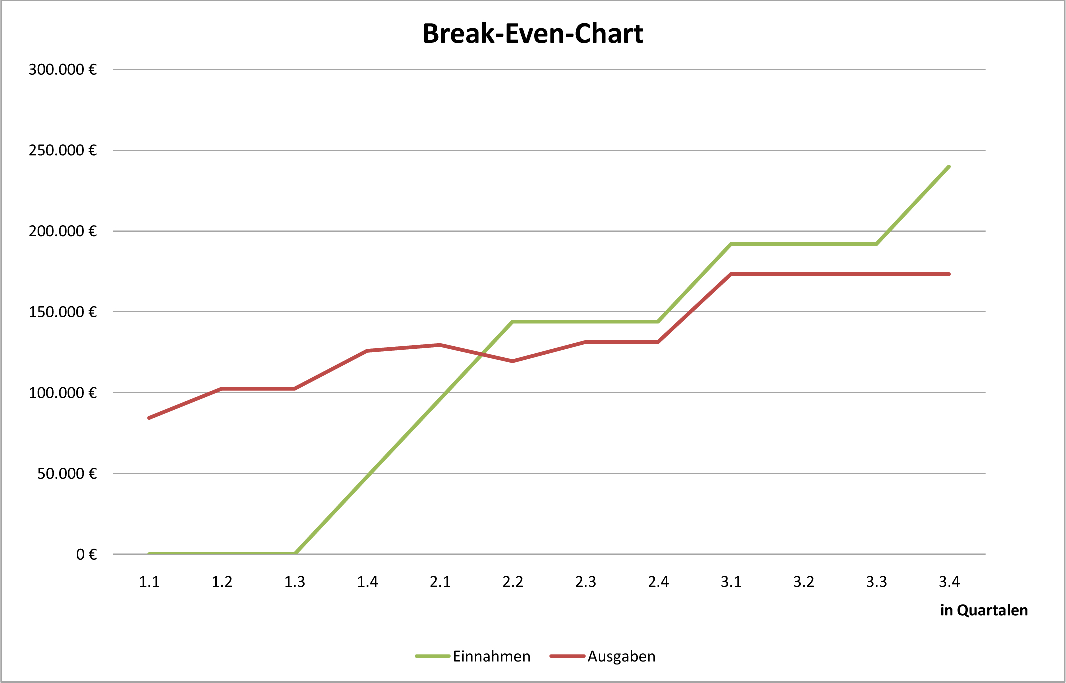
\includegraphics[width=0.8\linewidth]{../Bilder/BreakEvenChart}
\caption{Break-Even-Chart unseres Finanzplans}
\label{fig:BreakEvenChart}
\end{figure}
